\documentclass[11pt]{report}
\usepackage{graphicx}
\usepackage[a4paper, portrait, margin=1.6cm]{geometry}
\usepackage{enumitem}
\usepackage{lmodern}
\usepackage[T1]{fontenc}
\usepackage[hidelinks]{hyperref}
\newcommand{\ts}{\textsuperscript}

\begin{document}
\pagenumbering{gobble}
\hspace*{-\parindent}\hspace{-1em}
\begin{tabular}{p{3.8cm} p{13cm}}
    \vspace{0pt} 
    {%
	\setlength{\fboxsep}{0pt}%
	\setlength{\fboxrule}{0.75pt}%
    \fbox{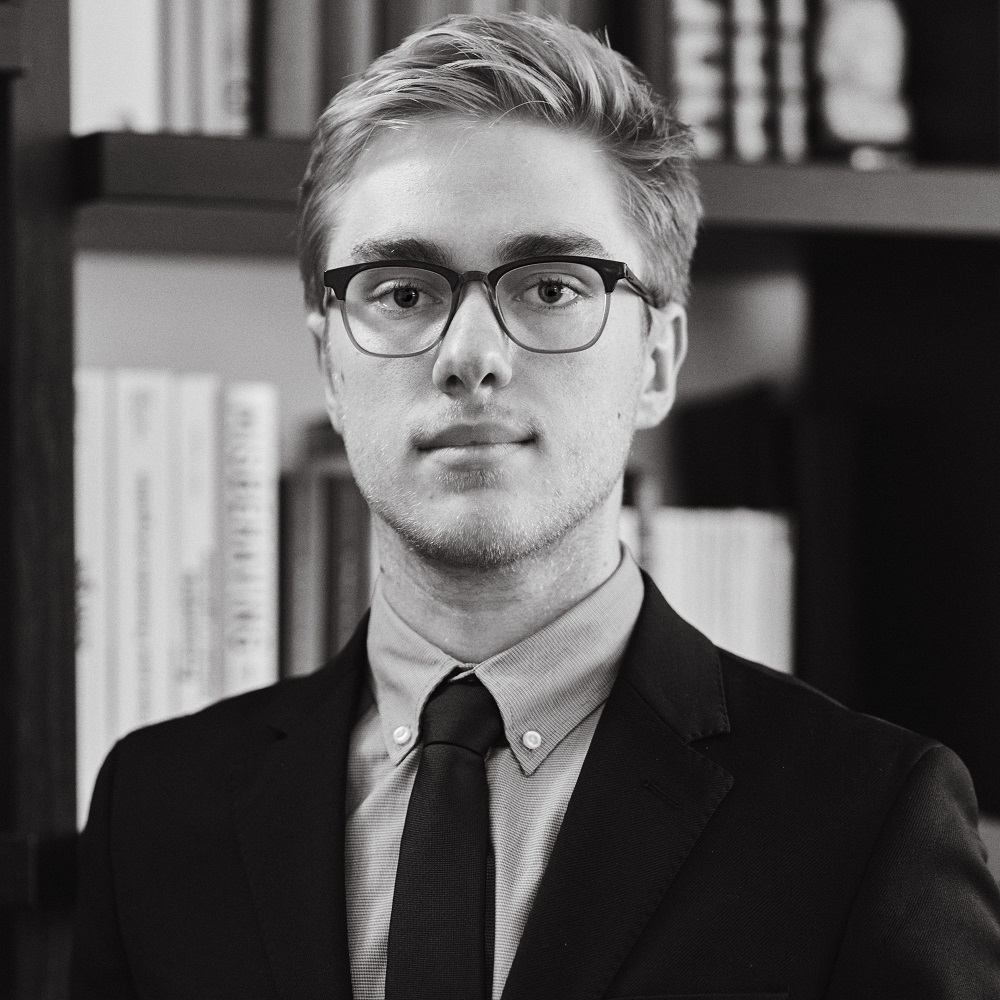
\includegraphics[scale=0.445]{picture.jpg}}%
    }%
    & 
    \vspace{0pt}
	\begin{Large}\textbf{PATRYK WISNIEWSKI}\end{Large}
	\newline \emph{Étudiant ingénieur économiste}
	\newline
	\newline Addresse: 155 Av. Pierre Brossolette, Montrouge, France
	\newline Courriel: \href{mailto:pa.wisniewski@proton.me}{\underline{pa.wisniewski@proton.me}}
	\newline Linkedin: \href{https://linkedin.com/in/pwisniewski02}{\underline{pwisniewski02}}
	\newline Phone: +33 6 95 30 31 18
	\newline Birthdate: 18/07/2002
	\end{tabular}

\begin{flushleft}
\raisebox{-.6ex}{FORMATION} \hrulefill
\end{flushleft}

	
\noindent\textbf{Programme ingénieur \textbar\space Économie et Statistiques}
\hfill
\textbf{08/2023 - present} \\
\emph{ENSAE - Institut Polytechnique de Paris}\\
Programme ingénieur multidisciplinaire combinant un niveau élevé de mathématiques appliquées, d'économie, d'informatique, de statistiques, d'économétrie et de machine learning. \\

\noindent\textbf{Master 1 \textbar\space Quantitative Economics}
\hfill
\textbf{08/2022 - 05/2023} \\
\emph{Université Paris Dauphine - PSL}\\
Master entièrement enseigné en anglais avec des cours avancés en microéconomie, macroéconomie, théorie des jeux et économétrie, ainsi que des enseignements supplémentaires en science des données. Projet de M1 sur l'économie de la vie privée et les asymétries d'informations entre individus et plateformes.\\
\\
\noindent\textbf{Licence \textbar\space Magistère d'Économie}
\hfill
\textbf{09/2019 - 06/2022} \\
\emph{Paris 1 Panthéon Sorbonne \& PSE}\\
Licence obtenue dans le magistère d'économie, un programme sélectif principalement axé sur les enseignements quantitatifs comprenant des mathématiques avancées, des statistiques et de l'économétrie. Mémoire sur l'effet de tremplin des contrats à court terme sur le marché du travail français.

	\begin{flushleft}
	\raisebox{-.6ex}{EXPÉRIENCES PROFESSIONNELLES} \hrulefill
	\end{flushleft}


\noindent\textbf{École des Mines de Paris} \hfill Paris, France\\[0.1cm]
\textbf{Stage recherche}\hfill \textbf{05/2023 - present} \\
Deuxième stage à l'etilab durant lequel j'ai eu l'occasion de travailler sur la création d'une topologie des entreprises de taille intermédiaires à l'aide de techniques d'apprentissage automatique. Durant mon stage j'ai également pu travailler sur la question des délais de paiements et du pouvoir de marché des eti. \\[0.15cm]
\textbf{Stage data et web}\hfill \textbf{06/2022 - 08/2022} \\
Stage au CERNA au sein de l'etilab, une chaire dédiée à l'étude des ETI d'Île-de-France. Pendant mon stage, j'ai pu développer une application web de visualisation (frontend et backend).
J'ai également pu ponctuellement prendre part à la collecte de données publiques et à la construction de la base de données. \\

\noindent\textbf{Narodowy Bank Polski} (Banque Centrale de Pologne) \hfill Varsovie, Pologne \\[0.1cm]
\textbf{Stage recherche}\hfill \textbf{05/2023 - present} \\
Stage à la Banque Centrale de Pologne durant lequel j'ai eu l'occasion de préparer une courte revue de littérature sur le policy-mix fiscal/monétaire en période d'inflation. J'ai également pu travailler avec d'autres stagiaires sur un modèle VAR des prix en période de pénurie. 

	\begin{flushleft}
	\raisebox{-.6ex}{COMPÉTENCES} \hrulefill
	\end{flushleft}



  \noindent\textbf{Languages de programmation :}\hfill{Java / Python / R / SQL / Matlab} \\
  \textbf{Productivité :}\hfill LaTeX / Microsoft Office / Git\\
  \textbf{Technologies Web :}\hfill JavaScript / HTML5 / CSS / nodeJS / PHP  \\
  \textbf{Administration systèmes :} \hfill Windows (advanced) / GNU Linux (intermediate)\\
  \textbf{Langues :} \hfill French (native) / Polish (native) / English (C1 - TOEFL 106/120) 

	\begin{flushleft}
	\raisebox{-.6ex}{LOISIRS} \hrulefill
	\end{flushleft}

\noindent Photographie argentique et numérique / Réparation d'éléctroniques / Réseaux et Hardware / Open Source


\end{document}

